\documentclass{standalone}
\special{background White}

\usepackage{tikz}
\usepackage{caption}
\usepackage{subcaption}
\usepackage{graphicx}
\begin{document}

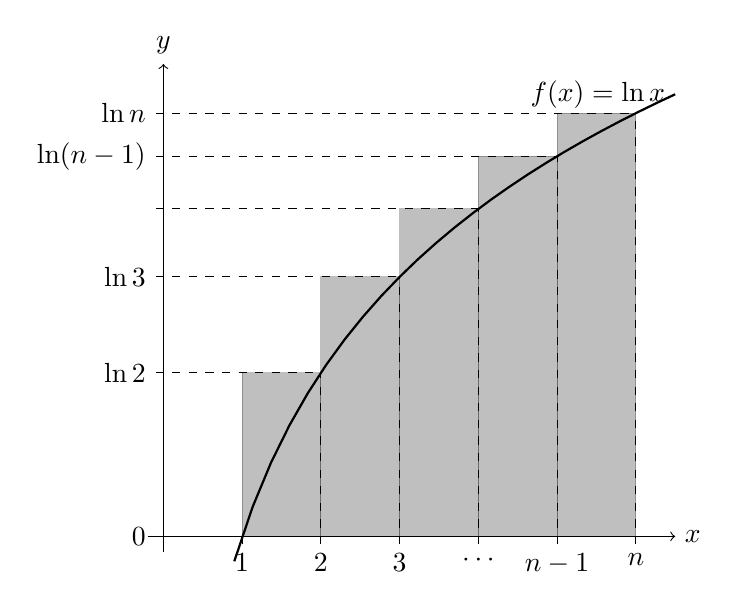
\begin{tikzpicture}[domain=0.9:6.5, scale=1]
    \tikzset{declare function={f(\x)=3 * ln(\x);}} %% define function
    % \draw[very thin,color=gray] (0,0) grid (8,8);

    \draw[->] (-0.2,0) -- (6.5,0) node[right] {$x$};
    \draw[->] (0,-0.2) -- (0,6) node[above] {$y$};

    \draw[thick]    plot (\x,{f(\x)})   node[left] {$f(x) =\ln x$};

    \foreach \x/\xtext/\ytext in {1/1/0,2/2/\ln 2,3/3/\ln3, 4/\cdots/ ,5/n-1/\ln(n-1),6/n/\ln n} {
            \draw[dashed] (\x,-0.1) node[below] {$\xtext$} -- (\x,{f(\x)}) ;
            \draw[dashed] (-0.1,{f(\x)}) node[left] {$\ytext$} -- (\x,{f(\x)});
            \filldraw [black, nearly transparent] ({\x-1},0) rectangle (\x,{f(\x)});
        }
\end{tikzpicture}
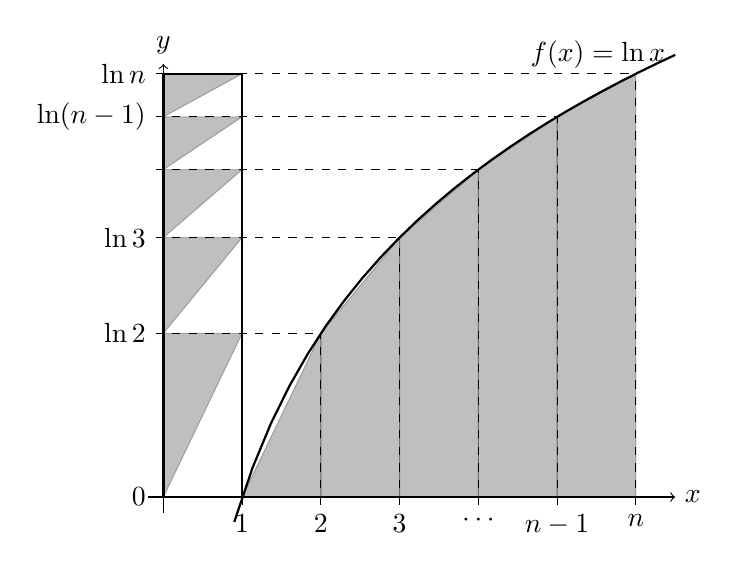
\begin{tikzpicture}[domain=0.9:6.5, scale=1]
    \tikzset{declare function={f(\x)=3 * ln(\x);}} %% define function
    % \draw[very thin,color=gray] (0,0) grid (8,8);

    \draw[->] (-0.2,0) -- (6.5,0) node[right] {$x$};
    \draw[->] (0,-0.2) -- (0,5.5) node[above] {$y$};

    \draw[thick]    plot (\x,{f(\x)})   node[left] {$f(x) =\ln x$};

    \foreach \x/\xtext/\ytext in {1/1/0,2/2/\ln 2,3/3/\ln3, 4/\cdots/ ,5/n-1/\ln(n-1),6/n/\ln n} {
            \draw[dashed] (\x,-0.1) node[below] {$\xtext$} -- (\x,{f(\x)}) ;
            \draw[dashed] (-0.1,{f(\x)}) node[left] {$\ytext$} -- (\x,{f(\x)});
            \ifnum \x<6
                \filldraw [black, nearly transparent] (\x,0) -- ({\x+1},0) -- ({\x+1},{f(\x+1)}) -- ({\x},{f(\x)}) -- cycle;
                \filldraw [black, nearly transparent] (0,{f(\x)}) -- (1,{f(\x+1)}) -- (0,{f(\x+1)}) -- cycle;
            \fi
    }
    \draw[thick]    rectangle (1,{f(6)});
\end{tikzpicture}

\end{document}